\begin{figure}[t]
    \centering
    \resizebox{0.9\textwidth}{!}{
    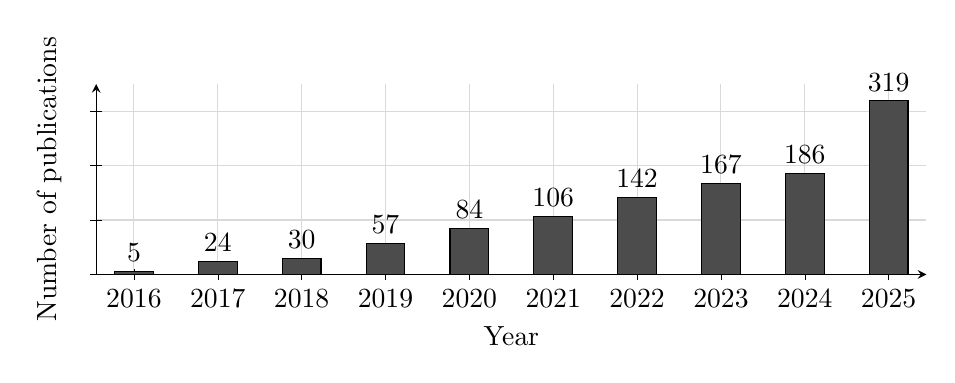
\begin{tikzpicture}
    \begin{axis}[
        width=\linewidth,
        height=4cm,
        ybar,
        bar width=14pt,
        ymin=0,
        ymax=350,
        yticklabels={},
        ylabel={Number of publications},
        xlabel={Year},
        symbolic x coords={2016,2017,2018,2019,2020,2021,2022,2023,2024,2025},
        nodes near coords,
        nodes near coords align={vertical},
        grid=both,
        major grid style={gray!30},
        minor grid style={gray!15},
        axis lines=left,
        tick style={black},
        enlarge x limits=0.05,
        title style={font=\bfseries},
    ]
    \addplot[
        fill=black!70
    ] coordinates {
        (2016,5)
        (2017,24)
        (2018,30)
        (2019,57)
        (2020,84)
        (2021,106)
        (2022,142)
        (2023,167)
        (2024,186)
        (2025,319)
    };
    \end{axis}
    \end{tikzpicture}
    }
    \caption{Yearly growth of Explainable Reinforcement Learning research with at least one citation on arXiv.}
    \label{fig:count_publications_xrl}
\end{figure}
